\section*{Introduction}

Compton scattering represents the main  type of $\gamma$-matter interaction with $\gamma$ energy of the MeV order.   
The aim of this report is to present the study of Compton Scattering performed with the experimental Set Up described in the following section.
This report will analyze these steps:
\begin{itemize}
	\item Energy calibration of the three inorganic scintillators.
	\item Verification of the relationship between energy and angle of the diffused photon.
	\item Measure of the differential cross section of Compton Scattering.
\end{itemize}

\section*{Experimental Set Up}

To study the Compton scattering three inorganic NaI(Tl) scintillators with 7.5~cm diameter and height were used~(see Fig.~\ref{Fig:Set_up}). A $^{22}$Na $\gamma$-source was positioned inside a collimator lead brick between the Tagger and Scatterer detectors, while the scattered photon Detector was placed on a rotating slide in order to select the desired scattering angle.

The last dinode outputs of the PMT were sent to a Quad Linear Gate FAN-IN/OUT mod. Philips 744 in order to split them. One output then was sent directly to a CAEN digitizer mod. DT5720, an ADC with a sampling rate of 250 Ms/s and a resolution of 12 bit, while the other ones were sent to a  CFTD module. The timing signals were needed to produce the coincidences between the three detectors through a 32 inputs Logic Units mod. LU 278. These signals were used as trigger input for the ADC unit.

\begin{figure}[h!]
	\centering
	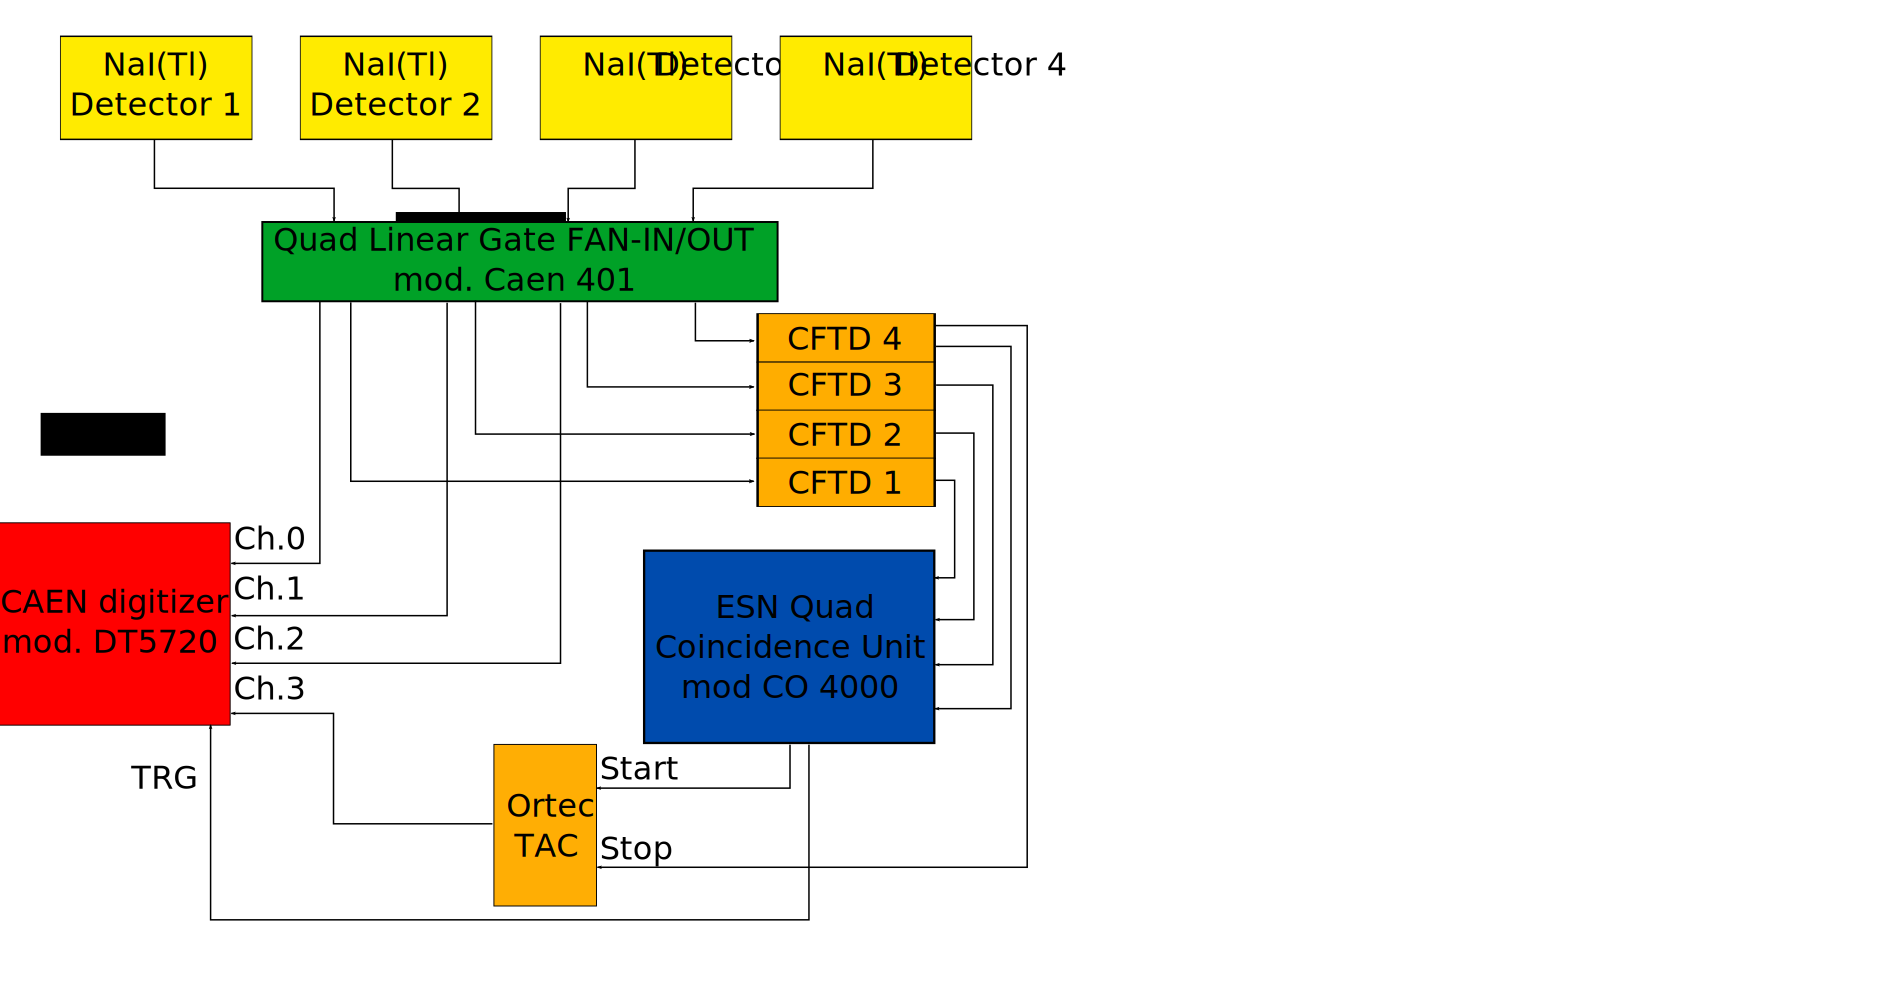
\includegraphics[width=\textwidth]{immagini/SetUp.pdf}
	\caption{Experimental configuration adopted for the Compton Scattering experiment.}
	\label{Fig:Set_up}
\end{figure}